\documentclass{article}
\usepackage[utf8]{inputenc}
\usepackage{float}
\usepackage{graphicx}
\usepackage{xcolor, soul}
\usepackage[english]{babel}
\usepackage[margin=1.7in]{geometry}
\bibliographystyle{unsrt}
\usepackage{hyperref}
\usepackage{amsmath}
\usepackage{amssymb}
\usepackage{subcaption}
\usepackage{mathtools}
\usepackage{tabularx,ragged2e,booktabs,caption,sidecap,subcaption,graphicx,tikz}

\begin{document}
\begin{titlepage}
	
	
	\title{Project 1 \\ Course 02445 \\ Project in Statistical evaluation of \\ artificial intelligence }
	\author{Rasmus J. P. s164564 \\ Nikolaj S. P. s183930}
	\date{January 2020}
	\maketitle
	
\subsection*{Summary}
Classifying trajectories is a complex problem with many dimensions. In this report we will attempt to classify trajectories with two different machine learning models, a neural network and the K-Nearest-Neighbors algorithm. We evaluated each model's performances on how well they classify trajectories on new observations and compared the performance of both models. We found a significant difference between model performances in favor of the neural network $\alpha < 0.01$. In addition we analyzed 16 different experiments and their resulting trajectories and tested whether there was a significant effect of experiment on trajectories. Using a multivariate test-statistics for high dimensional data we are able to conclude that 115/120 pairs of two-sample comparisons of means were significantly different than one-another $\alpha = 0.05$ and conclude that for the vast majority of the trajectories there will be an significant effect of the experiment being performed.

\end{titlepage}

\section{Introduction}
Solving complex problems has been the main drive for development in computer science and the computers has by far overceeded the humans on complex problems such as playing a game of chess or predicting the weather but only because we have been able to present them models simulating the real world for which the computer can react upon. So how do we model the real world? There are many answers, some complicated and some simple. We will be looking at trajectory data from 10 different test-subjects each performing 16 different experiments, repeated 10 times. Each experiment share the same underlying task with slight variation to the task. The task involved having human test-subjects move a cylinder over another cylinder. The experiments varied between different obstacle heights and obstacle positions. \\ Our first aim is to classify the supposed unique motion between test-subjects within the same experiment. The data from only a single experiment is then the 10 repetitions performed by each of the 10 test subjects, on which we will train and evaluate our models on. Sampling each model 30 times with leave-one-out cross validation LOOCV we will then compare the performance in a two-sampled t-test. \\Second aim is to look for a significant effect from the experiments on the trajectories. Since the data is multivariate we will test for multivariate normality and if the results are negative we turn to central limit theorem CLT and reduce our dataset to a dataset of 160 mean trajectories, 10 means for each experiment. Finally we compare mean trajectories by using a generalized form of the Student's t-statistic namely Hotelling's t-squared statistics "$t^{2}$ which generalizes to p-dimensionality.


\section{Data}
The trajectory \[motion\] data was recorded in 3 dimensions using a motion capture camera, resulting in three continuous variables x,y and z, furthermore the data included information about which person performed the motion, in which repetition the motion was captured and which experiments was performed thus giving us three categorical variables. \\ Each trajectory observation contains 100 recordings of said coordinates - see figure \ref{fig:trajectory}. \\Conveniently computers does not observe data like us humans, so we transform the motion data from 3 x 100 observations to 1 x 300, effectively stacking 300 coordinates along one vector and doing so we have not changed the premise of the problem.

\hl{Here goes motion plot traj}

\begin{figure}[H]
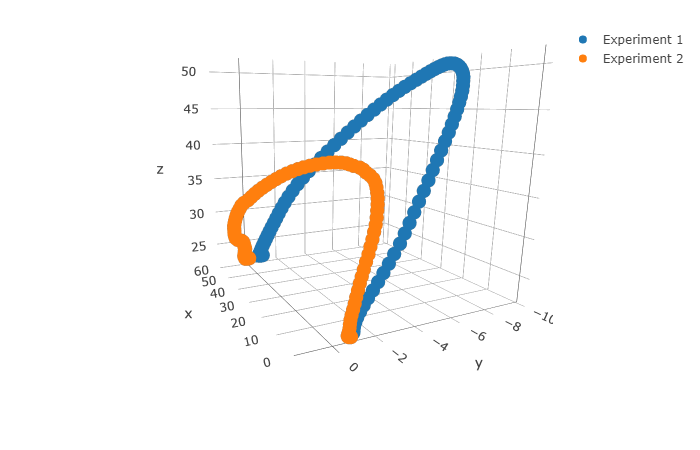
\includegraphics[width=\linewidth]{curve.png}
\caption{example of data}
\label{fig:trajectory}
\end{figure}


Subject 9 is missing the first 4 datapoints for some of the experiments, we will impute the values by replicating the first available datapoint, such that the first 5 datapoints become identical for those particular observation.

\hl{Here goes table for negative multivariate normality test}
TRAJ, variance between curves (boxplots), 

\section{Comparing classifiers}
We decided to compare two vastly different machine learning models, an ANN and a KNN, by running them multiple times and comparing the mean of our performance measure within each model. Performance measure was a simple measure of how many correct classification out of all possible. By training our models with the LOOCV algorithm, each fold only contains one test-entry, a measure of $"1"$ for a correct classification and $"0"$ for wrong classification was returned and all values summed after completion. We ran each model 30 times and by doing so recording 30 observations of a mean performance metric. CLT then tells us that these random variables will follow an approximate normal distribution and because of this fact we will be able to compare the two models by comparing the mean of their performance in a two-sampled Student's t-test.\\



We propose a null-hypothesis \fcolorbox{gray}{gray}{$H_{0}$: The difference between the means is equal to zero}. 
\subsection{Model A}
We experimented with several versions of ANNs to find the architecture best suited for the task. We decided to use an ANN because of their good performance on high dimensional data. The classification network was trained to classify a person from the 1 x 300 long vector of motion data. See a description of the ANN layout in table \ref{tab:ann}.

\begin{table}[H]
\centering
\begin{tabular}[H]{c l @{} l}
\centering
Layer no.       &
\multicolumn{2}{c}{Function} \\
\hline
Layer 1     & linear(300, 150) \\
            & ReLU \\
            & Dropout(0.15) \\
Layer 2     & linear(150, 75) \\ 
            & ReLU \\
            & Dropout(0.15) \\
Layer 3     & linear(75, 10) \\ 
Layer 4     & Softmax\\ 
\end{tabular}\\
\caption{Network parameters}
\label{tab:ann} 
\end{table}

\subsection{Model B}
The second model was a clustering model using the KNN algorithm, this model was trained on the same 1 x 300 motion vector.
The KNN was chosen because of its simplicity and because it is very cheap computationally, compared to other models such as the ANN.

\section{Testing the for experimental influence}
Our variables needs to be normally distributed within an experiment to use the test-statistic. We tested our variables if they were normally distributed and found that only 12 out of the 300 were for all of the experiments. When comparing the experiments we would need to use the same variables, we would be limited to those 12 and need to removed the majority of the data, and at that point the comparison would no longer make sense to make.

If an experiment were to have a significant effect on the resulting trajectories, it should be significantly different from any other trajectory. The multiple test statistics to asses is then a collection of 120 comparisons i.a all possible combination of a single pair of experiments - duplicates and pairs of the same experiments removed.\\ 
This proposed test statistics raises two important points concerning our data:
\begin{enumerate}
	\item  Are the 100 repetitions within experiments multivariate \textbf{normally} distributed?
	\item Having only 100 observations per experiment we are limited to less than 200 explaining variables per Hotelling's T-squared statistcs $p < n_x + n_y -1$ where p is the dimensions in the multivariate observations.
\end{enumerate}

The second point quickly becomes less of an issue, we will reduce the dimensionality of our data using principal component analysis PCA and choosing the number of principal components PCs by analyzing the square roots of the resulting eigenvalues i.e analyzing the variance explained by the eigenvectors. But first we must solve the multivariate normal assumption. \\
 We have enough observations to assume normal distribution but we should only do this within single test subjects, and in fact it shows that the vast majority of variables are normally distributed individually see \ref{tab:normality} but, we cannot expect the motion of one subject in a test to be identical to another subject's motion and thus we are forced to reduce our data to one mean observation per subject per experiment. Another problem then arises, we have just reduced our data set from a large set of 1600 individual observation to a mere 160 and when we compare two experiments the number is even lower at only 10 observation, down from 100 and the scenario is that we now must limit ourselves to a maximum of nine \hl{19?} explaining variables, down from 99 \hl{199} before calculating means. \hl{Whhoouv ... actually nx+ny-1 variables are allowed in two-sampled T-squared test}\\
 This loss of data is made up for by the 82\% variance explained by the first 9 PCs. We project the matrix of means onto the rotation matrix returned from PCA. To sum it up, the reason for this detour was that testing for normality i.e multivariate normality, returned negative, the very same test which found single variables to be normally distributed did not find the 100 observation within an experiment to be of a multivariate normal distribution hence why we must turn to CLT and somehow find mean test statistics.\\
The Hotelling's T-squared statistics is a generalized version of the Student's t statistic. It generalizes to \textit{p} dimensions. We again propose a null-hypothesis of no difference in between the means of trajectories from different experiments. 

\section{Results}
LOOCV was performed 30 times to get a good estimate of the variance of the generalization accuracy of the two classification models, from this a confidence interval was calculated \ref{tab:CI.acc}. Table \ref{tab:CI.acc} show the confidence intervals for both the ANN and the KNN model, the first value in second column is the generalized accuracy measure i.e estimated percentage of successful classification. Adding and subtracting the second value from the first in the second column return the 95\% confidence intervals. We see that the two intervals does not overlap, provided a 0.95 confidence level.

\begin{minipage}{\linewidth}
\centering
\captionof{table}{Confidence interval of classifiers} 
\begin{tabular}{ c c}\toprule[2pt]
\bf Model  & \bf CI of Generalization Accuracy \\\midrule[1.5pt]
ANN  & $0.708 \pm 0.0078$  \\\midrule
KNN  & $0.644 \pm 0.0066$ \\
\bottomrule[1.25pt]
\end {tabular}\par
\label{tab:CI.acc}
\end{minipage} \bigskip

\begin{minipage}{\linewidth}
	\centering
	\captionof{table}{Two-sampled paired comparison of means} 
	\begin{tabular}{ c c c}\toprule[1.5pt]
	\bf Test  & \bf Test Statistic & \bf p-value \\\midrule[1.5pt]
	Paired t-test  & $10.934$ &  $8e-12$ \\
	\bottomrule[1.5pt]
	\end {tabular}\par
	\label{tab:ml.test}
\end{minipage} \bigskip

The same story follows from the paired test seen in table \ref{tab:ml.test}. We notice a very high test score of $10.934$ and subsequently the resulting p-value which is approximately zero. The very reason for such high test score is that all 30 observations per model each come from the LOOCV algorithm were we effectively train and test on all the data available and the resulting values will be very close to equal which gives us very little variance also evident from the small confidence interval in table \ref{tab:CI.acc} as a result we can with very high confidence say that difference in performance between the two model is not zero and that the artificial neural network is the better classifier.

Testing for effect on trajectories from experiments we compared 120 unique pairs of two experiments resulting in the confusion matrix in figure \ref{fig:confusion}. The matrix shows 120 p-values representing the performed comparison between the experiment from the row against the experiment from the row. With a significance level $alpha = 0.05$ we see a large amount of significant entries $p-value < 0.05$ - colored in blue and only a handful to be excact of non-significant entries $p-value \leq 0.05$ - colored red. Interestingly must non-significant observation, 3/5, comes from the setup of "S" small height of obstacle, and then a combination of short to medium-short distance to obstacle.

\begin{minipage}{\linewidth}
\centering
\captionof{table}{Non-significant pairs of Experiments}
\begin{tabular}{cc}\toprule[1.5pt]
\textbf{Experiment pair} & \textbf{p-value} \\\midrule[1.25pt]
1, 4         	& 0.137            \\\midrule
4, 7  		& 0.177            \\\midrule
7, 10           	& 0.278            \\\midrule
5, 8        	& 0.0855           \\\midrule
6, 9      	& 0.162           \\\bottomrule[1.25pt]
\end{tabular}
\label{tab:sig}
\end{minipage}

\section{Appendix}





\end{document}